% Collision data, MC samples and reweightings
\section{Collision Data}
\label{mc:sec:coldata}

All events that pass the trigger (Sec.~\ref{sec:det:trigger}) are assigned to a data stream, which is saved to disk for further analysis. For example, the ``Egamma'' stream contains events that passed at least one of the electron or photon triggers, while the ``JetEtMiss'' stream contains events with jets or missing transverse energy. An event that contains both a jet and an electron can be saved in both streams. Naturally, this analysis utilizes the ``Muon'' stream, which contains about 440 million events in total.

Data collected throughout 2011 is separated into 11 data periods (B, D-M). A new period is started when significant changes occur in operating conditions (such as the introduction of a new trigger menu), or after a technical shutdown. The transition from period B to period D involved a particularly significant change in conditions: the time spacing between bunch collisions was decreased from 75 ns to 50 ns. Because 50 ns bunch spacing was preserved for the rest of the year, period B with its abnormal bunch spacing was dropped entirely from this analysis, resulting in a small data loss on the order of 0.7\%.

The amount of data collected at collider experiments is described through the concept of luminosity. Instantaneous luminosity measures the flux, which has the units of the number of particles per unit time per unit area: $cm^{-2} s^{-1}$. Integrating the flux over a period of time, we obtain integrated luminosity in units of $cm^{-2}$. However, in order to keep the numbers manageable, high energy physicists use an alternative unit of area: barn. By definition, 1 barn is $10^{-24}~cm^2$, which is approximately equal to the cross-sectional area of uranium. Integrated luminosity is then expressed in units of inverse-barns, usually $fb^{-1}$.

Cross-sections of various processes are expressed in units of area (usually $nb$). Multiplying cross-section by integrated luminosity produces the expected number of process events in a given amount of collected data. 

Fig.~\ref{fig:mc:lumi} shows the total integrated luminosity collected throughout 2011, as a function of the day of the year.

\begin{figure}[phtb]
  \begin{center}
    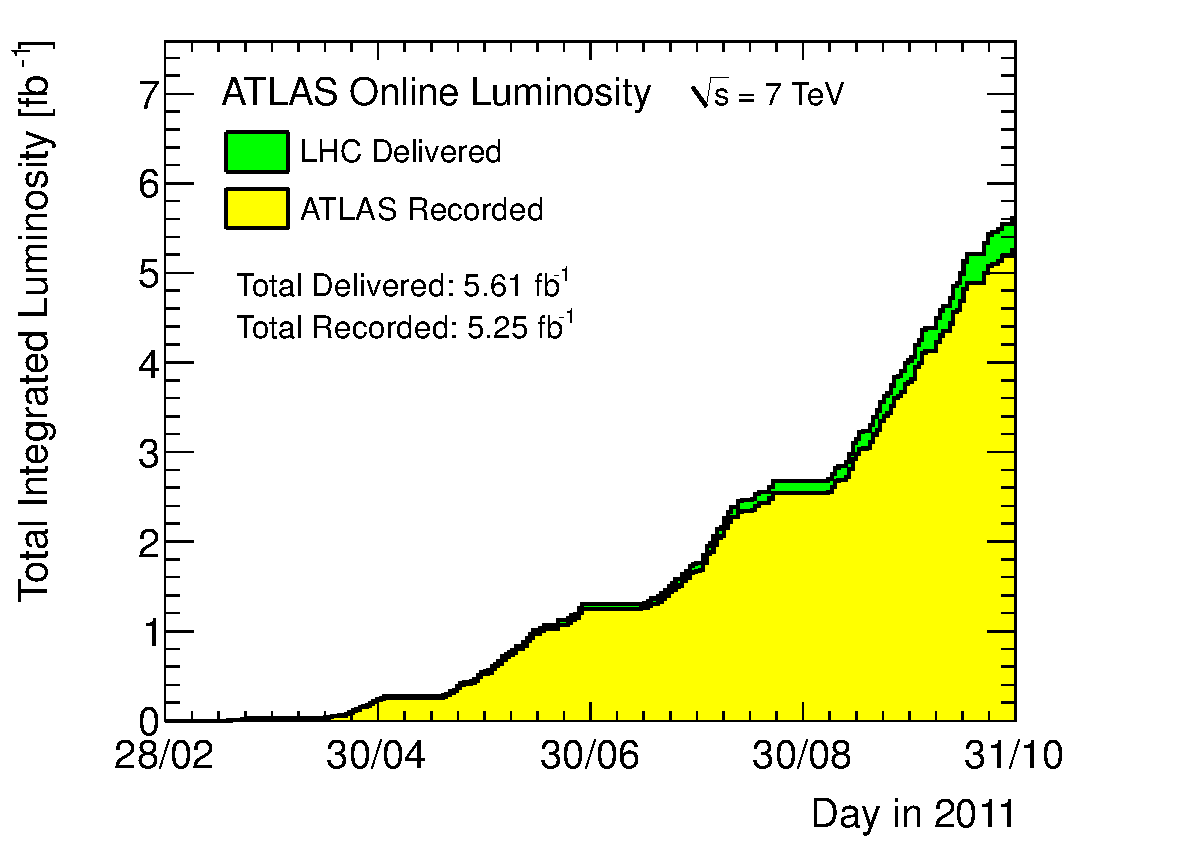
\includegraphics[width=0.7\textwidth]{mc/fig/sumLumiByDay}
    \caption{ Integrated luminosity in 2011 as a function of the day of the year.}
    \label{fig:mc:lumi}
 \end{center}
\end{figure}

The data considered in this analysis has a total integrated luminosity of \lumitr\ with a systematic uncertainty of $1.8\%$~\cite{ATLAS-CONF-2012-080}. The integrated luminosity figure is smaller than the $5.25$ $fb^{-1}$ recorded by ATLAS because data collected in suboptimal conditions was removed from the analysis.

\section{Monte-Carlo Samples}
Monte-Carlo simulation plays a crucial role in this analysis. It serves two purposes: to estimate and subtract the backgrounds to \Wmn\ decay, and to ``unfold'' the measured distributions to a detector-independent cross-section, as outlined in Sec.~\ref{sec:xsec_formula}.

Monte-Carlo events are produced through a series of steps:
\begin{itemize}
\item \textbf{Generation} - creates a list of four-vectors of all stable particles produced in a proton-proton collision. Generators calculate scattering amplitudes, perform parton showering and hadronization, and include the emissions from the underlying event. In the ATLAS simulation framework, the output of all generators is interfaced with two additional programs: \Photos~\cite{Golonka:2005pn}, which simulates the final state QED radiation, and \Tauola~\cite{Jadach:1990mz}, which decays polarized $\tau$ leptons.
\item \textbf{Simulation} - propagates all final state particles through the ATLAS detector using the GEANT4 toolkit~\cite{geant4}, which includes a detailed treatment of the interaction of particles with the material in the detector. GEANT4 relies on a comprehensive model of the detector, which includes everything from bulk material to individual mounting brackets.
\item \textbf{Digitization} - converts the energy depositions left in the detector into digital values seen by the readout electronics. In addition, the effect of multiple proton-proton interactions per bunch crossing (pileup) is simulated by overlaying the so-called minimum bias events on the original hard scattering interaction. Minimum bias events model the average detector response from a typical proton-proton collision, unbiased by resonant processes. LHC run conditions prevalent in 2011 produced around 10 additional pileup interactions per bunch crossing.
\item \textbf{Reconstruction} - takes digitized event data and identifies and reconstructs all particles (muons, jets, et cetera) in the event. Reconstruction software at ATLAS consists of a large collection of packages fine-tuned over the years using test beam studies and the LHC data. The same reconstruction algorithms run on Monte-Carlo simulation and real detector data.
\end{itemize}

Generation is the most interesting step because it is closely related to theory and depends on the modeling of non-perturbative parts of QCD calculations, such as PDFs or parton showers. In this analysis, the following generator programs are used for signal and background samples:

\begin{itemize}
\item \Powheg~(Positive Weight Hardest Emission Generator)~\cite{Nason:2004rx,Frixione:2007vw,Alioli:2008gx,Alioli:2010xd} - an NLO generator used for \Wmn\ and \Zmm\ samples. For parton showering, \Powheg\ can be interfaced with \Pythia~\cite{pythia} or \Herwig~\cite{Corcella:2000bw} programs. \Pythia\ showering is used by default, while \Herwig\ provides a systematic variation.
\item \Mcatnlo~\cite{mcatnlo} - an alternative NLO generator used to produce systematic variations of \Wmn\ and \Zmm\, as well as $t\bar{t}$ and single top samples. Unlike \Powheg, \Mcatnlo\ generates a subset of events with negative weights (about 10\% of the total) that combine with positive-weight events to enforce NLO accuracy. \Mcatnlo\ can be interfaced only with \Herwig\ for showering.
\item \Herwig~\cite{Corcella:2000bw} - a general-purpose generator used both for matrix element calculations and parton showering in diboson samples.
\item \Alpgen~\cite{Mangano:2002ea} - a generator that specializes in multi-parton processes by computing the full matrix element of configurations with additional emissions. It was used for $W\to\tau\nu$ and $\Zg \to \tau\tau$ samples because the more traditional \Pythia-based $\tau$ samples have limited statistics and suffer from incorrect treatment of $\tau$ polarization.
\end{itemize}

All NLO Monte-Carlo samples are interfaced with the \pdfCteq\ PDF set.

\subsection{List of Samples and their Cross-Sections}

Table~\ref{tab:samples} contains a full list of Monte-Carlo samples used in this analysis. For each sample, the table provides its cross-section times the branching ratio times the filter efficiency (pre-selection efficiency at the generator level), and the total number of simulated events.

Electroweak processes are normalized to the NNLO cross-sections computed with the FEWZ program~\cite{Gavin:2010az, Gavin:2012sy, Li:2012wn}. The uncertainty on these cross-sections arises from the choice of PDF (3\%) and factorization and renormalization scales.

\begin{table}[p]
  \small
  \begin{center}
    \begin{tabular}{l|l|r|r}
      \hline
      \hline
      \raisebox{-0.4ex}{Process} & Generator & $\sigma{\cdot}
      \text{BR}{\cdot}\epsilon_{filter}$ [nb] & $N_{evt}\,[10^6]$\\
      \hline\hline

      \multicolumn{3}{c}{Signal samples for \Wln}\\\hline
      \Wplusmunu     &  \Powheg\Pythia  & 6.16 (5\%) & 23 \\
      \Wminusmunu    &  \Powheg\Pythia  & 4.30 (5\%) & 17 \\
      \Wplusmunu     & \Powheg\Herwig   & 6.16 (5\%) & 16 \\
      \Wminusmunu    & \Powheg\Herwig   & 4.30 (5\%) & 12 \\
      \Wplusmunu     & \Mcatnlo & 6.16 (5\%) & 16 \\
      \Wminusmunu    & \Mcatnlo & 4.30 (5\%) & 12 \\

      \hline \multicolumn{3}{c}{\Zgll\ samples}\\\hline
      \Zgll ~~($\mll > 53.8\gev$) &   \Powheg\Pythia   &  1.01 (5\%) & 20\\
      \Zgll ~~($\mll < 53.8\gev$)  &  \Powheg\Pythia   &  0.088 (5\%) & 3\\

      \hline \multicolumn{3}{c}{\Alpgen\Herwig\  and \Sherpa\ \Wln\ and \Zgll\ samples}\\\hline
      \Wtau\ Np0   &   \Alpgen\Herwig\ & 8.29 (5\%) & 3.4 \\
      \Wtau\ Np1   &   \Alpgen\Herwig\ & 1.56 (5\%) & 2.5 \\
      \Wtau\ Np2   &   \Alpgen\Herwig\ & 0.45 (5\%) & 3.8 \\
      \Wtau\ Np3   &   \Alpgen\Herwig\ & 0.12 (5\%) & 1 \\
      \Wtau\ Np4   &   \Alpgen\Herwig\ & 0.03 (5\%) & 0.25 \\
      \Wtau\ Np5   &   \Alpgen\Herwig\ & 0.008 (5\%) & 0.07 \\

      \Ztau\ Np0  &  \Alpgen\Herwig\  & 0.83 (5\%) & 6.6 \\
      \Ztau\ Np1  &  \Alpgen\Herwig\  & 0.17 (5\%) & 1.3 \\
      \Ztau\ Np2  &  \Alpgen\Herwig\  & 0.051 (5\%) & 0.81 \\
      \Ztau\ Np3  &  \Alpgen\Herwig\  & 0.014 (5\%) & 0.22 \\
      \Ztau\ Np4  &  \Alpgen\Herwig\  & 0.004 (5\%) & 0.06 \\
      \Ztau\ Np5  &  \Alpgen\Herwig\  & 0.0009 (5\%) & 0.02 \\

      \hline \multicolumn{3}{c}{$t\bar{t}$ and single top samples}\\\hline
      $t\bar{t}$   & \Mcatnlo & 0.098 (6.2\%) & 1.5\\
      single top, $t$ chan  & \Mcatnlo & $7.12\cdot 10^{-3}$ (12\%) & 0.3\\
      single top, $s$ chan & \Mcatnlo & $0.47\cdot 10^{-3}$ (12\%) & 0.3\\
      single top, $Wt$ chan & \Mcatnlo & $14.59\cdot 10^{-3}$ (12\%) & 0.9\\

      \hline \multicolumn{3}{c}{Diboson samples}\\\hline
      $WW$ & \Herwig & 17.5 $\cdot 10^{-3}$ (7\%) & 1.5 \\
      $WZ$ & \Herwig & 5.7 $\cdot 10^{-3}$ (7\%) & 1 \\
      $ZZ$ & \Herwig & 1.3 $\cdot 10^{-3}$ (7\%) & 0.25 \\

      \hline \multicolumn{3}{c}{QCD samples (for cross-checks only)}\\\hline
      $b\overline{b}$ ($p_{T, \mu} > 15\gev$) & \Pythia & $73.9$ & 4.5\\
      $c\overline{c}$ ($p_{T, \mu} > 15\gev$) & \Pythia & $28.4$ & 1.5\\

      \hline\hline
    \end{tabular}
    \caption{ Monte-Carlo samples used in the analysis. The numbers in the parentheses next to cross-section values indicate the uncertainty on these cross-sections. The quoted cross-sections are the ones used to normalize the estimates of expected Monte-Carlo event counts. }
    \label{tab:samples}
  \end{center}
\end{table}

\section{Theoretical Extrapolation Tables}
\label{sec:mc:extraptables}
The extrapolation (\E) and acceptance (\A) factors (defined in Sec.~\ref{sec:xsec_formula}) are derived from \Wmn\ Monte-Carlo. Four sources of systematic uncertainty are considered when assigning errors to \E\ and \A\ factors:
\begin{itemize}
\item The uncertainty envelope of the default CT10 parton distribution function (PDF) family. PDF's assign a fraction of the total proton momentum to the quarks or gluons that interact to produce a \Wboson\ boson. These distributions are not calculable from first principles and are measured experimentally, mostly from proton-electron scattering experiments. A more detailed discussion is available in the theory section~\ref{chap:pdf_theory}.
\item Variations arising from using alternative NLO (next-to-leading order) PDF families. There are several NLO PDF families maintained by various research groups, each emphasizing different experimental inputs or fitting techniques to derive parton distributions. The maximum deviation between the default CT10 family and one of the following PDF families is taken as the uncertainty:
\begin{itemize}
\item ABM11 NLO~\cite{Alekhin:2012ig}
\item HERAPDF 1.5 NLO~\cite{Aaron:2009aa,Radescu:2011cn}
\item MSTW2008 NLO~\cite{Martin:2009iq}
\item NNPDF2.3~\cite{Ball:2012cx}
\end{itemize}
\item Variations arising from using an alternative Matrix Element (ME) Monte-Carlo generator. Matrix elements involve the ``hard'' (high-$p_{T}$) part of the interaction that can be calculated in perturbative QCD through Feynman diagrams. Differences between Monte-Carlo generators arise in the specific implementation, particularly once these calculations go beyond the leading order. Further details are available in Sec.~\ref{chap:qcd_theory}. The ME uncertainty is taken as the difference between the \Mcatnlo\ and \Powheg\ generators.
\item Variations arising from using alternative Parton Shower (PS) mechanisms in the Monte-Carlo. Parton showering simulates additional emissions from particles produced in the hard scattering, including soft gluon emissions. The PS uncertainty is taken as the difference between \Herwig\ and \Pythia\ showering.
\end{itemize}

Central values and uncertainties on \E\ and \A\ factors and shown in Tables~\ref{tab:ae_w_int}~-~\ref{tab:ae_w_etaptdiff}. These numbers were derived by the inclusive W/Z analysis group.

\begin{table}
  \footnotesize
  \centering
  \begin{tabular}{|c|r|r|r|r|r|r|}
    \hline
    & ~~Value~~
    & ~~$\Delta_\mathrm{CT10} [\%]$~~
    & $\Delta_\mathrm{PDFmax} [\%]$
    & ~~$\Delta_\mathrm{ME} [\%]$~~
    & ~~$\Delta_\mathrm{PS} [\%]$~~
    & ~~$\Delta_\mathrm{tot} [\%]$~~ \\\hline
    \multicolumn{7}{|l|}{\EW\ \Wmn\ fiducial ($|\eta|<2.4$) to fiducial/extrapolated ($|\eta|<2.5$) } \\
    \hline
    $\Wminus$ & $0.9682$ & $0.07$ & $-0.14$ & $-0.01$ & $-0.03$ & $0.16$\\
    $\Wplus$ & $0.9628$ & $0.06$ & $0.06$ & $-0.00$ & $-0.05$ & $0.09$\\
    \hline
    \multicolumn{7}{|l|}{\AW\ \Wmn\ fiducial/extrapolated to total} \\
    \hline
    $\Wminus$ & $0.4488$ & $0.80$ & $-1.60$ & $-0.62$ & $-0.83$ & $2.07$\\
    $\Wplus$ & $0.4645$ & $0.51$ & $1.11$ & $-0.39$ & $-0.80$ & $1.51$\\
    \hline
  \end{tabular}
  \caption{\AW\ and \EW\ factors and their relative uncertainties for the integrated \Wmn\ measurement.}
  \label{tab:ae_w_int}
\end{table}

\begin{table}
  \footnotesize
  \centering
  \begin{tabular}{|c|c|r|r|r|r|r|r|}
    \hline
    $|\eta|_\mathrm{min}$
    & $|\eta|_\mathrm{max}$
    & ~~Value~~
    & ~~$\Delta_\mathrm{CT10} [\%]$~~
    & $\Delta_\mathrm{PDFmax} [\%]$
    & ~~$\Delta_\mathrm{ME} [\%]$~~
    & ~~$\Delta_\mathrm{PS} [\%]$~~
    & ~~$\Delta_\mathrm{tot} [\%]$~~ \\\hline
    \multicolumn{8}{|l|}{\EW\ \Wminusmunu\ fiducial ($|\eta|<2.4$)
      to fiducial/extrapolated ($|\eta|<2.5$)} \\\hline
    $2.18$ & $2.50$ & $0.6982$ & $0.11$ & $-0.29$ & $0.01$ & $-0.00$ & $0.31$\\
    \hline
    \multicolumn{8}{|l|}{\EW\ \Wplusmunu\ fiducial ($|\eta|<2.4$)
      to fiducial/extrapolated ($|\eta|<2.5$)} \\\hline
    $2.18$ & $2.50$ & $0.6976$ & $0.08$ & $0.24$ & $0.07$ & $-0.11$ & $0.29$\\
  \hline
  \end{tabular}
  \caption{\EW\ factors and their relative uncertainties for the 1D $\eta$ differential \Wmn\ measurements. Because \EW\ factors merely extrapolate the measurement from $|\eta|<2.4$ to $|\eta|<2.5$, they are only needed for the most forward measurement bin. }
  \label{tab:ae_w_etadiff2}
\end{table}

\begin{table}
  \footnotesize
  \centering
  \begin{tabular}{|c|c|c|c|r|r|r|r|r|r|}
    \hline
    $|\eta|_\mathrm{min}$
    & $|\eta|_\mathrm{max}$
    & $p_{T, \mathrm{min}}$
    & $p_{T, \mathrm{max}}$
    & ~~Value~~
    & $\Delta_\mathrm{CT10} [\%]$
    & $\Delta_\mathrm{PDFmax} [\%]$
    & $\Delta_\mathrm{ME} [\%]$
    & $\Delta_\mathrm{PS} [\%]$
    & $\Delta_\mathrm{tot} [\%]$ \\\hline
    \multicolumn{10}{|l|}{\EW\ \Wminusmunu\ fiducial ($|\eta|<2.4$)
      to fiducial/extrapolated ($|\eta|<2.5$)} \\\hline
$2.18$ & $2.50$ & $20.0$ & $25.0$ & $0.6929$ & $0.10$ & $0.40$ & $0.30$ & $0.08$ & $0.51$\\
$2.18$ & $2.50$ & $25.0$ & $30.0$ & $0.6946$ & $0.10$ & $0.15$ & $0.13$ & $-0.01$ & $0.23$\\
$2.18$ & $2.50$ & $30.0$ & $35.0$ & $0.6964$ & $0.11$ & $-0.25$ & $-0.18$ & $-0.04$ & $0.33$\\
$2.18$ & $2.50$ & $35.0$ & $40.0$ & $0.6973$ & $0.12$ & $-0.35$ & $-0.07$ & $-0.03$ & $0.37$\\
$2.18$ & $2.50$ & $40.0$ & $45.0$ & $0.6993$ & $0.13$ & $-0.37$ & $0.04$ & $-0.14$ & $0.42$\\
$2.18$ & $2.50$ & $45.0$ & $50.0$ & $0.7041$ & $0.12$ & $-0.37$ & $0.58$ & $0.55$ & $0.89$\\
$2.18$ & $2.50$ & $50.0$ & $120.0$ & $0.7097$ & $0.13$ & $-0.36$ & $0.31$ & $0.25$ & $0.55$\\
  \hline
    \multicolumn{10}{|l|}{\EW\ \Wplusmunu\ fiducial ($|\eta|<2.4$)
      to fiducial/extrapolated ($|\eta|<2.5$)} \\\hline
$2.18$ & $2.50$ & $20.0$ & $25.0$ & $0.7172$ & $0.09$ & $0.36$ & $0.19$ & $-0.04$ & $0.42$\\
$2.18$ & $2.50$ & $25.0$ & $30.0$ & $0.7057$ & $0.09$ & $0.24$ & $0.22$ & $-0.19$ & $0.39$\\
$2.18$ & $2.50$ & $30.0$ & $35.0$ & $0.6971$ & $0.09$ & $0.20$ & $0.09$ & $-0.08$ & $0.25$\\
$2.18$ & $2.50$ & $35.0$ & $40.0$ & $0.6939$ & $0.09$ & $0.26$ & $0.19$ & $-0.03$ & $0.33$\\
$2.18$ & $2.50$ & $40.0$ & $45.0$ & $0.6925$ & $0.09$ & $-0.28$ & $0.04$ & $-0.38$ & $0.48$\\
$2.18$ & $2.50$ & $45.0$ & $50.0$ & $0.7000$ & $0.09$ & $1.08$ & $-0.92$ & $0.25$ & $1.44$\\
$2.18$ & $2.50$ & $50.0$ & $120.0$ & $0.7097$ & $0.09$ & $0.22$ & $-0.64$ & $-0.06$ & $0.68$\\
  \hline
  \end{tabular}
  \caption{\EW\ factors and their relative uncertainties for the 2D $\eta - p_T$ differential \Wmn\ measurement. Because \EW\ factors merely extrapolate the measurement from $|\eta|<2.4$ to $|\eta|<2.5$, they are only needed for the most forward measurement bin. }
  \label{tab:ae_w_etaptdiff}
\end{table}


\section{Monte-Carlo Corrections}
Several corrections are applied to Monte-Carlo samples to improve the modeling of relevant physics processes and detector conditions. Note that the data-driven corrections to muon momentum and reconstruction efficiency are described separately in the section on muon performance (Sec.~\ref{sec:event:muonperf}).

\subsection{Pile-up Reweighting }
% https://twiki.cern.ch/twiki/bin/view/AtlasPublic/LuminosityPublicResults#2011_pp_Collisions
The effect of multiple proton-proton interactions per bunch crossing (pileup) is accounted for in Monte-Carlo at the digitization step. However, the number of minimum-bias events overlaid in digitization does not exactly match the actual data taking conditions. Consequently, a pileup reweighting is applied as a function of $<\mu>$, the mean number of interactions per bunch crossing.
Fig.~\ref{fig:mc:nvtx} shows a comparison of the number of vertices with at least three tracks before and after pileup reweighting. The number of vertices acts as a proxy for the number of interactions because each $pp$ interaction produces a separate vertex that can normally be identified by looking at vertex positions along the $z$ axis. Pileup reweighting markedly improves the data/MC agreement.

\begin{figure}[phtb]
  \begin{center}
        \subfigure[Before pileup reweighting]{%
          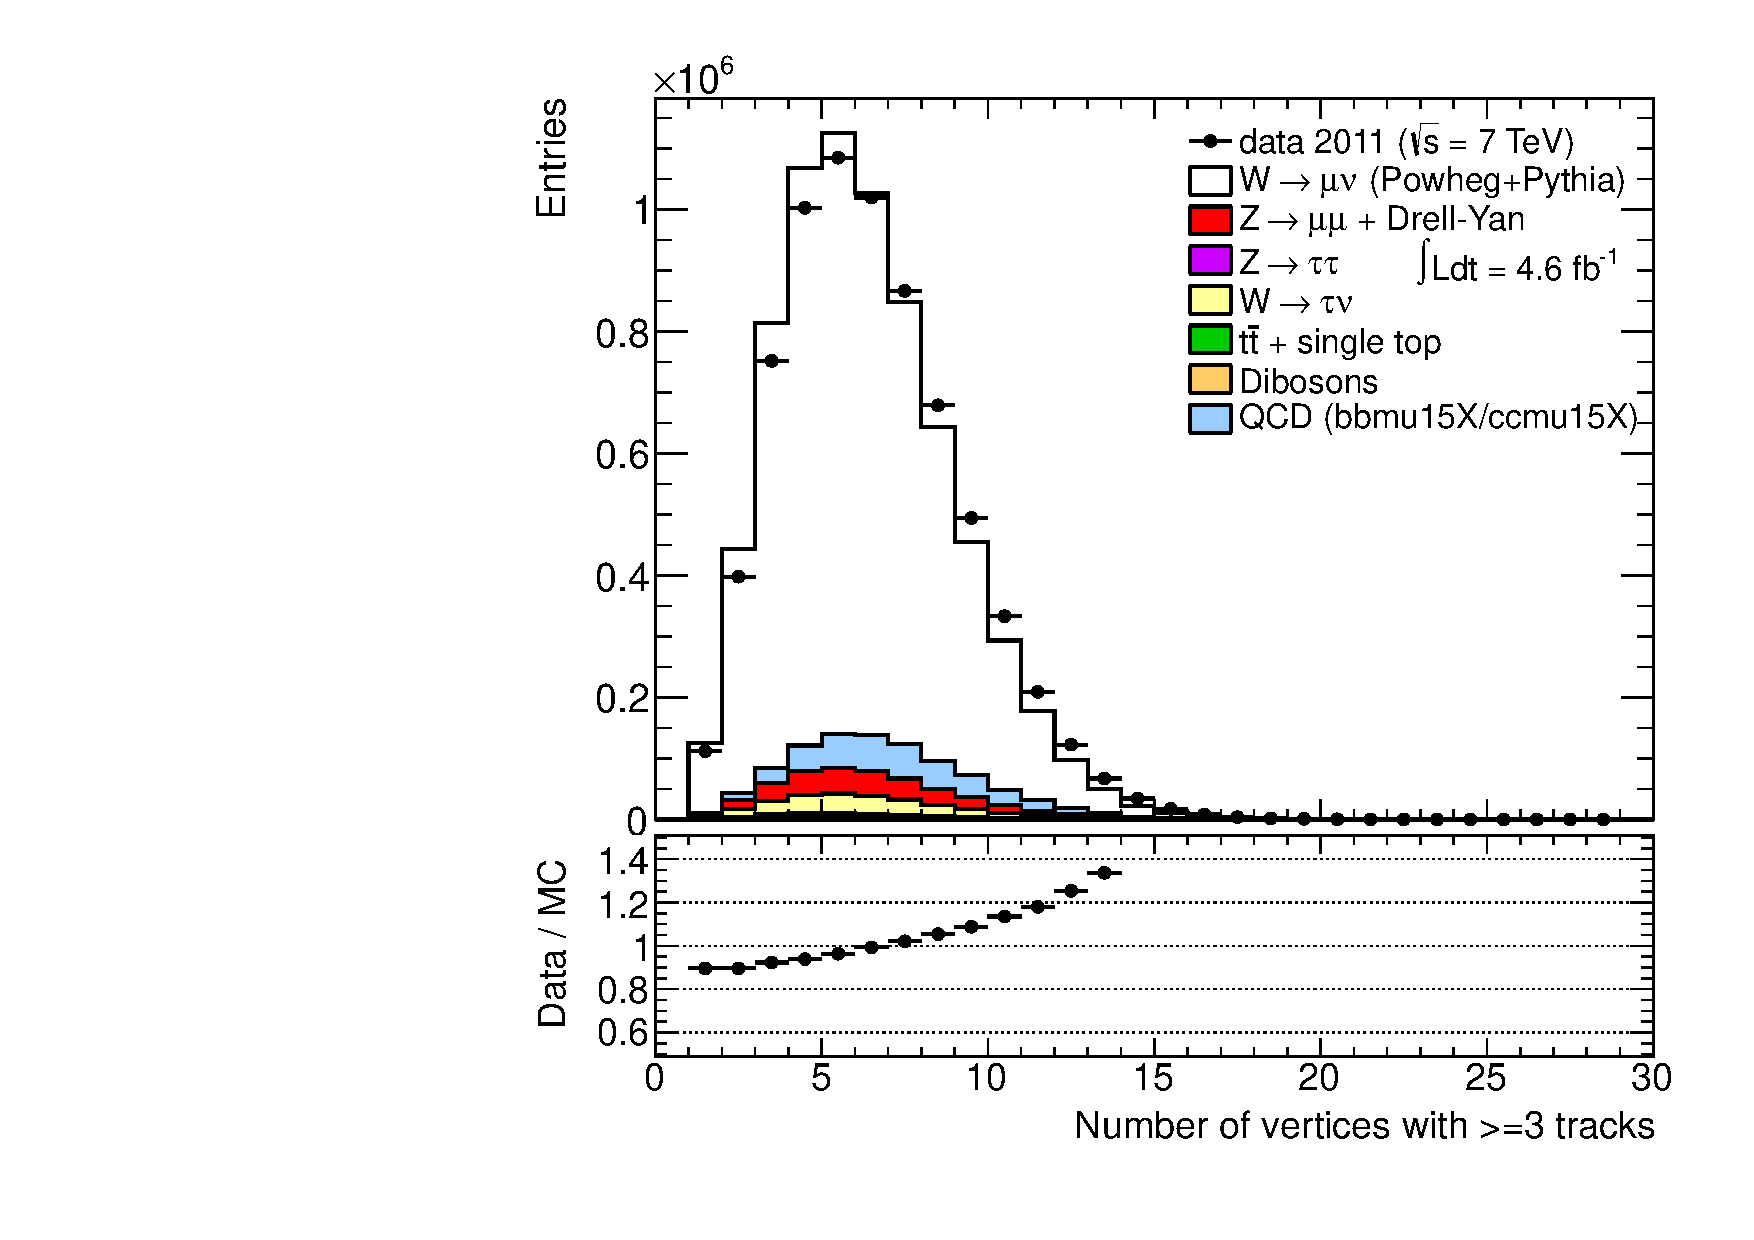
\includegraphics[width=0.44\textwidth]{mc/fig/rw_nvtx_pre}
        } 
        \subfigure[After pileup reweighting]{%
          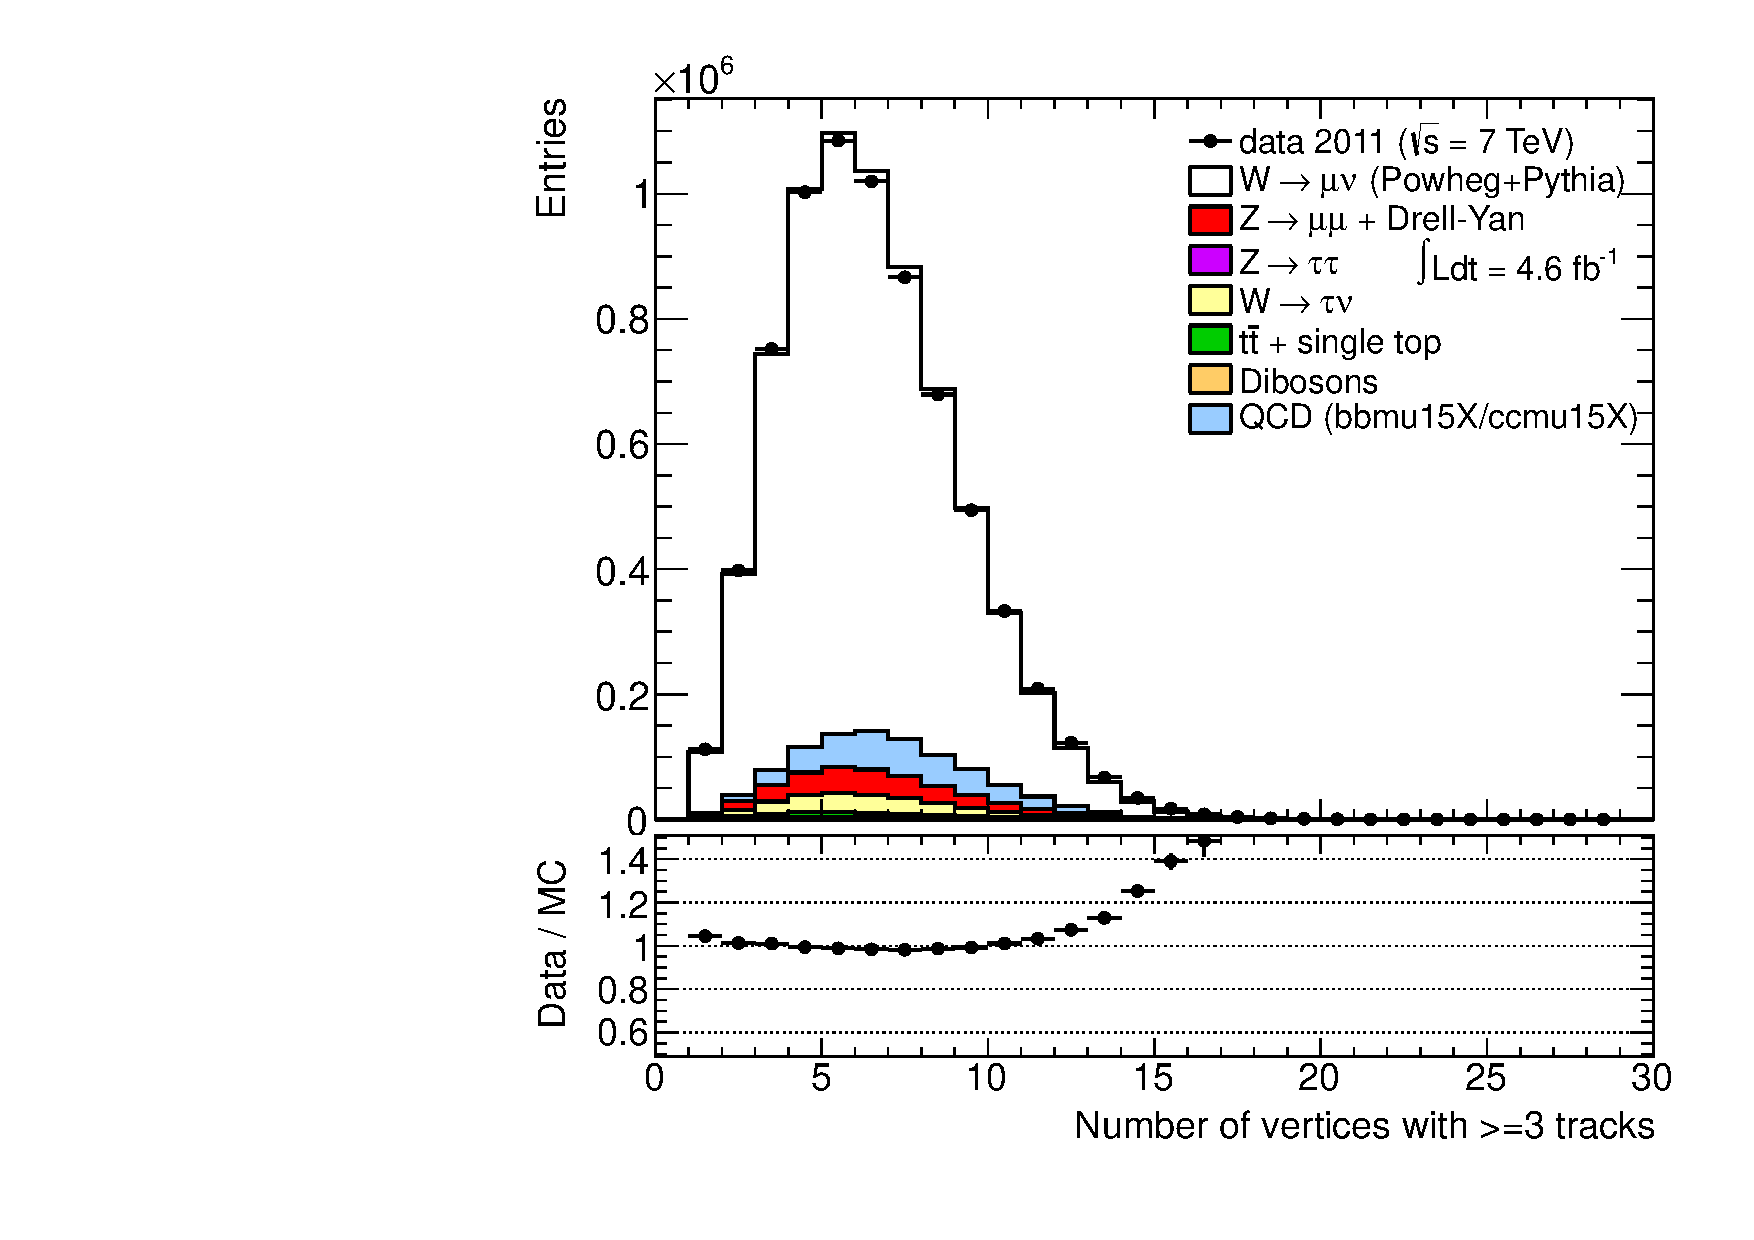
\includegraphics[width=0.44\textwidth]{mc/fig/rw_nvtx_aft}
        }
 \caption{ Distribution of the number of vertices with 3 tracks or more with and without pileup reweighting. Because of residual disagreement even after reweighting, an additional systematic on pileup modeling is introduced in the analysis by scaling the $<\mu>$ distribution by 3\%.}
 \label{fig:mc:nvtx}
 \end{center}
\end{figure}

\subsection{Vertex z Reweighting }
The spread of the beam spot along the $z$ direction is not well modeled in Monte-Carlo. This is corrected by applying a weight to Monte-Carlo at the truth level. Fig.~\ref{fig:mc:vxz0} shows the primary vertex $z_0$ distribution before and after reweighting.

\begin{figure}[phtb]
  \begin{center}
        \subfigure[Before vertex reweighting]{%
          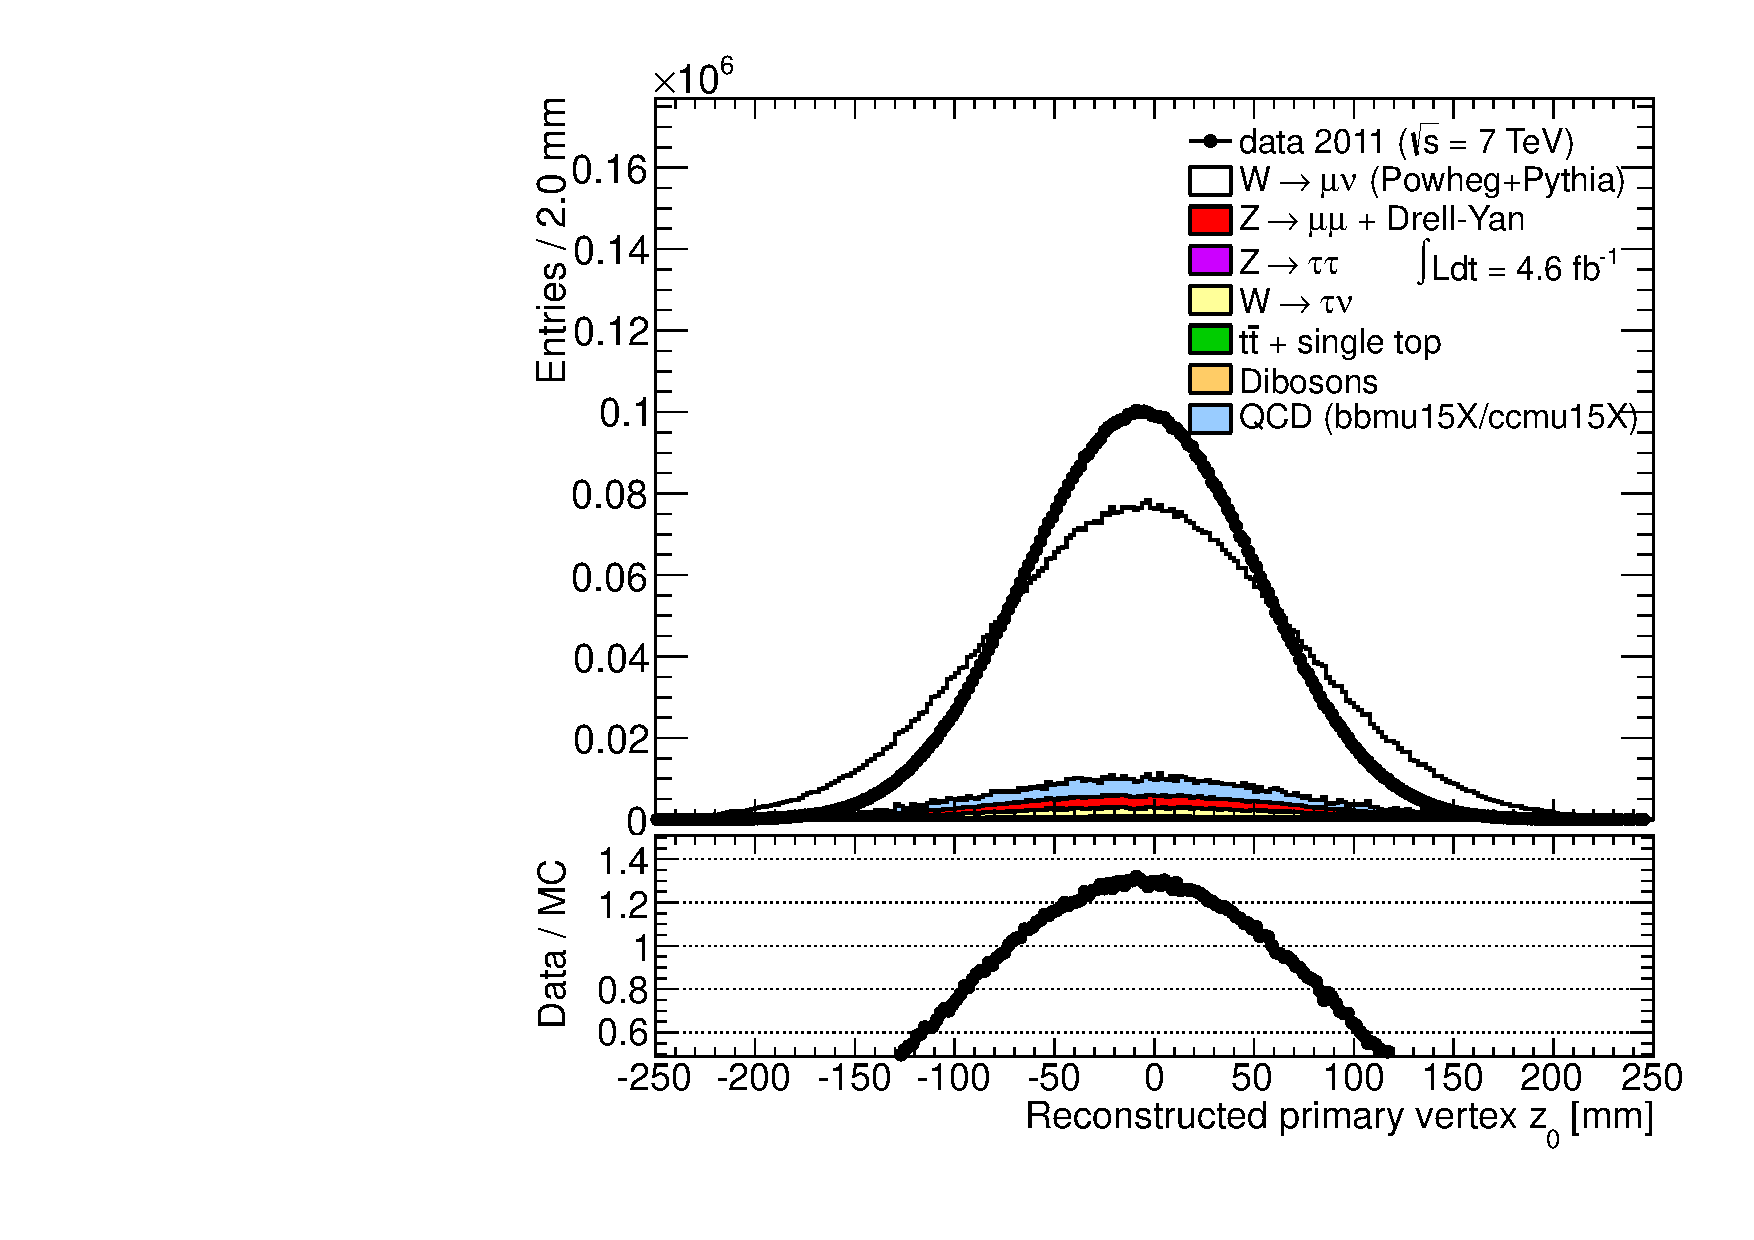
\includegraphics[width=0.44\textwidth]{mc/fig/rw_vxz0_pre}
        } 
        \subfigure[After vertex reweighting]{%
          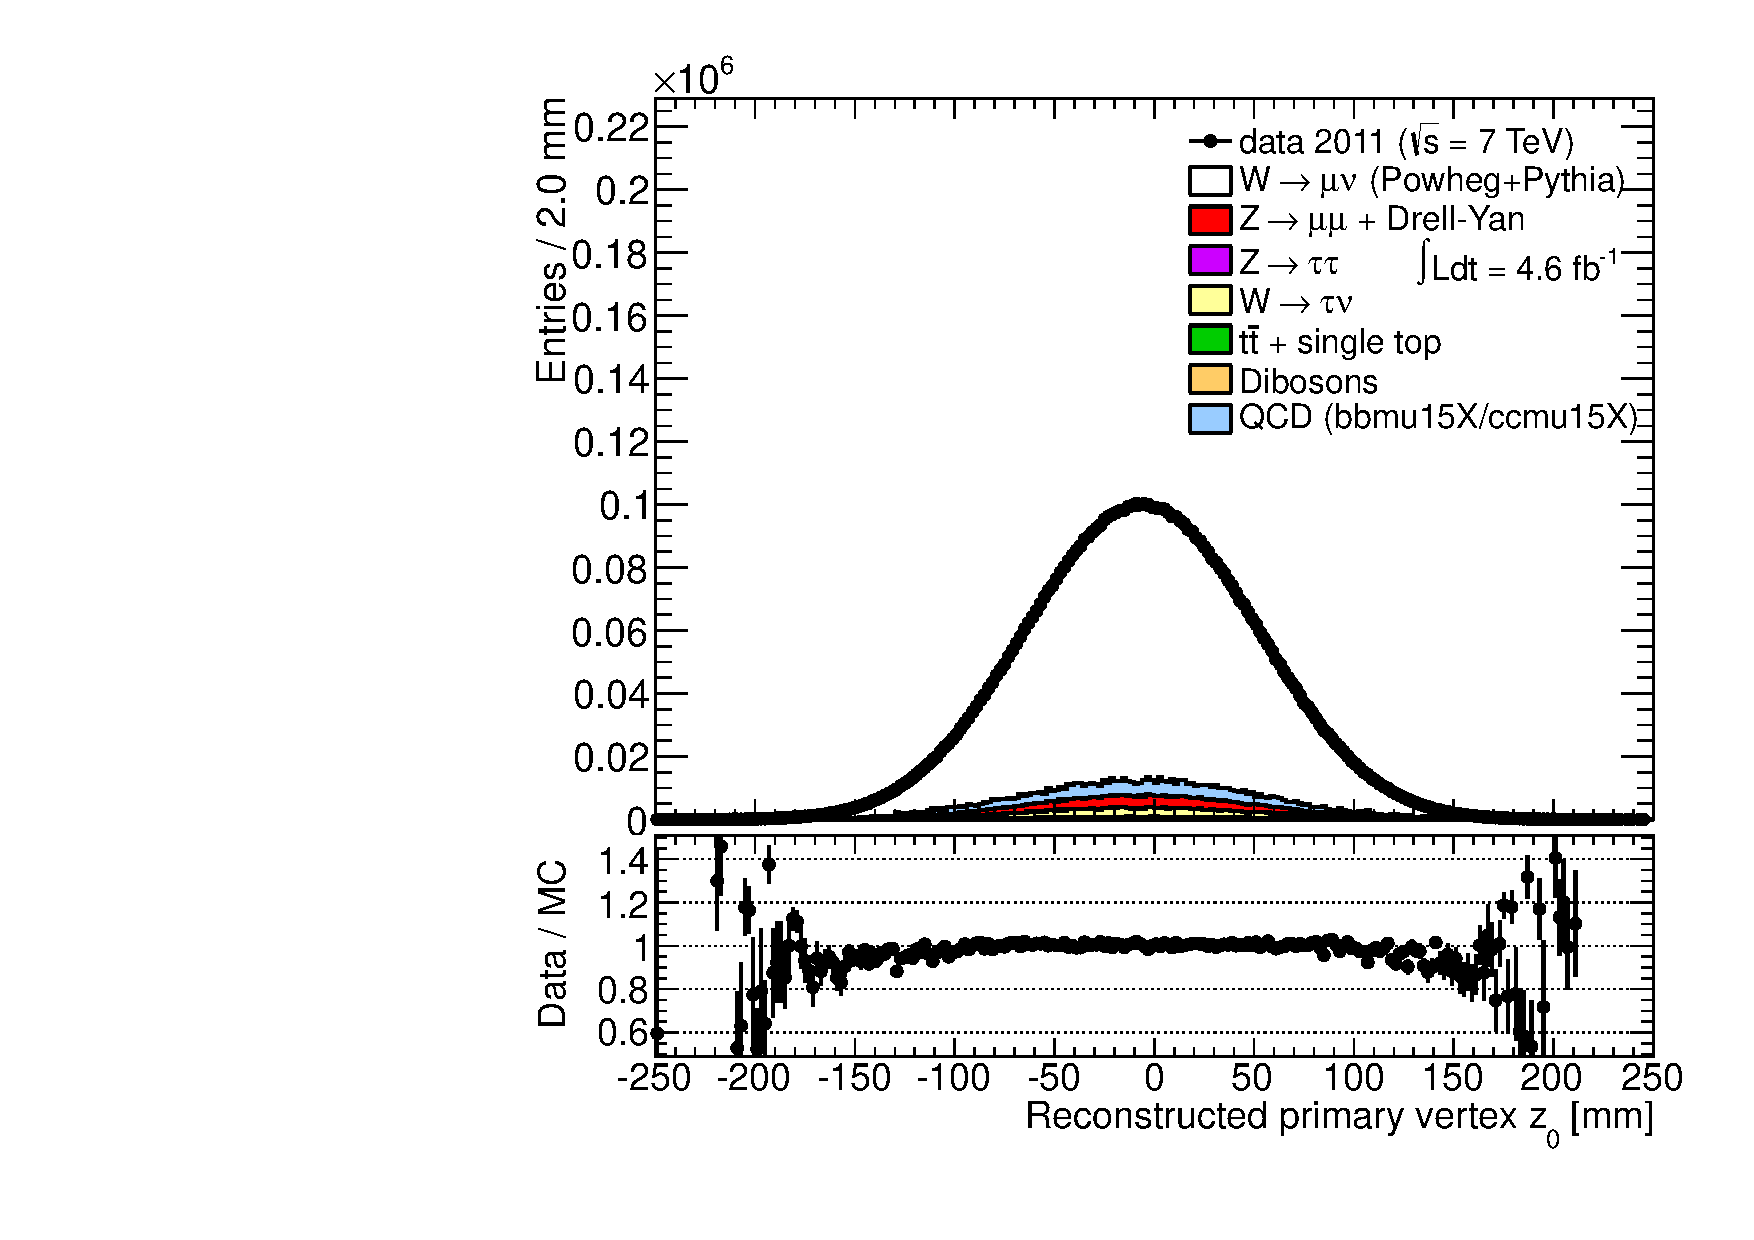
\includegraphics[width=0.44\textwidth]{mc/fig/rw_vxz0_aft}
        }
 \caption{ Primary vertex $z_0$ with and without vertex reweighting. }
 \label{fig:mc:vxz0}
 \end{center}
\end{figure}


\subsection{W and Z $p_T$ Reweighting }
\label{sec:bosonptreweight}
Published ATLAS $Z$ $\phi^*$ and $\pt$ analyses~\cite{Aad:2011fp} suggest that the boson $p_T$ spectrum is not correctly modeled by existing NLO generators. For example, \Fig~\ref{fig:zphistar_mcplot} from~\cite{zphistar} shows that none of the generators attain good data/MC agreement in the $Z$ $\phi^*$ variable, which is highly correlated to boson $p_T$ via $\phi^* \sim p_{T,\ell\ell}/\mll \approx p_{T,\ell\ell}/100\gev$. Therefore, for the nominal measurement, W and Z boson $p_T$ is reweighted in \Powheg\Pythia, \Powheg\Herwig, and \Mcatnlo\ samples to the published Z $p_T$ spectrum~\cite{Aad:2011gj}. The reweighting is based on the measured Z $p_T$ (rather than W $p_T$) because of concerns about hadronic recoil in the W case. Reweighting to \Sherpa\ and \Powheg\Pythiaeight\ is used to assess the systematic uncertainty.

\begin{figure}[htb]
  \begin{center}
    \includegraphics[width=0.9\textwidth]{MCReweights/zphistar_fig_03}
    \caption{Comparison of different MC generators to the $Z$ $\phi^*$ measurement using 2011 ATLAS data.}
    \label{fig:zphistar_mcplot}
  \end{center}
\end{figure}

\subsection{W and Z Lineshape Reweighting }
Generators used to produce \Wln\ and \Zgll\ samples differ in some of their settings, such as the mass and width of the gauge bosons, the form of the resonance parametrization, and the choice of couplings. A set of weights was developed~\cite{iba_maarten_vicini} to reweight each generator to a more optimal ``Improved Born Approximation''. For example, Fig.~\ref{fig:bosonm_reweight} demonstrates that the Z lineshapes of two different Monte-Carlo generators can be brought to a good agreement following the reweighting.

\begin{figure}[htb]
  \begin{center}
    \subfigure[Before \Zgll\ LineShape Reweight]{%
      \includegraphics[width=0.45\textwidth]{MCReweights/zgamma_pythia_powheg_std}
    }%
    \subfigure[After \Zgll\ LineShape Reweight]{%
      \includegraphics[width=0.45\textwidth]{MCReweights/zgamma_pythia_powheg_rew}
    } \\
    \caption{Effect of lineshape reweighting on the ratio of \Pythia\ and \Powheg\Pythia. Agreement is achieved following reweighting to the ``Improved Born Approximation'' set of parameters. In this particular case, most of the improvement comes from the \Powheg\Pythia\ side.}
    \label{fig:bosonm_reweight}
  \end{center}
\end{figure}

%% \subsection{Alpgen Angular Reweighting }
%% \Alpgen\Herwig\ $W\to\tau\nu$ and $\Zg\to\tau\tau$ samples do not model boson rapidity $y$ well due to the fact that they rely on a sub-optimal leading-order PDF (\pdfCteql). The weights are derived by comparing the nominal samples with samples reweighted to \pdfCteq.

\subsection{PDF reweighting}

The authors of PDF families provide uncertainties on the fitted momentum fractions through a set of PDF ``members'' that deviate from the nominal PDF by moving along error eigenvectors. For example, the CT10 family contains 52 members, making it impractical to re-run the full Monte-Carlo chain for each member.
As an alternative, PDF reweighting is applied to the nominal Monte-Carlo samples. For each event, the information stored in the truth record is used to calculate the weight via:
\begin{equation}
  w = \frac{xf_1^\mathrm{new}(x_1, Q^2_1) xf_2^\mathrm{new}(x_2, Q^2_2) }{xf_1^\mathrm{old}(x_1, Q^2_1) xf_2^\mathrm{old}(x_2, Q^2_2)}\,
\end{equation}
where $xf_i^\mathrm{new(old)}(x,Q^2)$ are the PDFs of the incoming
parton $i$ evaluated at a given Bjorken $x$ and scale $Q^2$ of the new
(old) PDF set~\cite{Bourilkov:2006cj}.
PDF reweighting is facilitated through the LHAPDF package~\cite{Whalley:2005nh}.
